% partes/parte2/cap09.tex
\chapter{Base tecnológica para el análisis del recorrido}
\label{cap:09}

\begin{cajaFicha}
\begin{description}
  \item[Unidad temática] II — Proceso de toma de decisión de compra digital.
  \item[Temas del programa] 2.4 Base tecnológica para el análisis del proceso de compra digital y \textit{customer journey}: 2.4.1 Temas selectos de buscadores y plataformas de gestión integral, redes sociales y comercio electrónico.
  \item[Horas] Teoría 2.0 · Práctica 3.0 · Aprendizaje autónomo 2.0 (asignación tentativa; ver Anexo B del prompt de proyecto, anomalía 4).
  \item[Competencia de la unidad] Examina el proceso de toma de decisiones de compra del consumidor digital a partir de su recorrido y figuras participantes.
  \item[Resultados de aprendizaje observables] Al concluir el capítulo, el estudiante:
  \begin{enumerate}
    \item ubica cuatro categorías de herramienta en las capas de captura, identidad, análisis y activación;
    \item evalúa una herramienta con criterios durables (cobertura del recorrido, privacidad y consentimiento, interoperabilidad, costo) sin depender de una marca;
    \item obtiene pesos de criterios con AHP y comprueba si sus juicios son consistentes;
    \item ordena alternativas con TOPSIS y localiza el peso en que cambia la elección.
  \end{enumerate}
  \item[Prerrequisitos] Cap. 1--8.
\end{description}
\end{cajaFicha}

\section{Caso de apertura}

\textbf{Vigente a octubre de 2026.} El Cap.~4 comenzó con dos predicciones que
no se cumplieron. Este capítulo parte de un hecho documentado. La versión
anterior de Google Analytics, Universal Analytics, dejó de procesar datos
nuevos el 1 de julio de 2023, y el 1 de julio de 2024 se perdió el acceso a
su interfaz y a su API \parencite{google2026ga4ua}. Quien construyó su
medición del recorrido sobre esa herramienta tuvo que rehacerla, y quien la
había atado a sus informes sin exportar los datos perdió el histórico.

\begin{casoFicticio}
Una tienda en línea mexicana contrata una herramienta de grabación de sesiones
porque \enquote{permite ver lo que hace el cliente}. Siete meses después,
una auditoría interna descubre que la herramienta también grabó lo que las
personas escribían en el formulario de pago. La tienda no sabía que podía
excluir esos campos, no pidió consentimiento específico y no puede exportar
las grabaciones para borrarlas con facilidad.
\end{casoFicticio}

Los dos casos tienen la misma moraleja. La herramienta que \emph{hoy} analiza
el recorrido es una decisión con consecuencias de privacidad,
interoperabilidad y costo que se pagan después. Por eso este capítulo no
presenta un catálogo de marcas, que envejecería antes de la próxima edición.
Presenta criterios y un método para aplicarlos.

\section{Desarrollo teórico}

\subsection{Temas selectos: cuatro capas y cuatro categorías de herramienta}
\progtag{2.4.1}
\label{sec:cap09-capas}

El programa deja abierto este subtema (\enquote{temas selectos}) por la
misma razón que el Cap.~4: el panorama cambia más rápido que un libro. La
estructura que sí perdura es la de las capas por las que pasa un dato del
recorrido (figura~\ref{fig:cap09-capas}): se \emph{captura}, se \emph{asocia a una
identidad}, se \emph{analiza} y se \emph{activa} en algún canal. Cada
categoría de herramienta opera sobre una o varias capas.

\begin{figure}[!htb]
  \centering
  \resizebox{0.95\textwidth}{!}{% figuras/tikz/cap09-pila-analitica.tex
% Cuatro capas de la base tecnológica para analizar el recorrido y las
% categorías de herramienta que operan en cada una. Criterios, no marcas.
\begin{tikzpicture}[
    capa/.style={rectangle, rounded corners, draw=guindaIPN, thick, fill=guindaIPNClara,
                 minimum width=11.5cm, minimum height=1.25cm, align=left, font=\scriptsize, text width=11.0cm},
    cat/.style={rectangle, rounded corners, draw=bronceIPN, thick, fill=bronceIPNClaro,
                minimum width=3.9cm, minimum height=1.25cm, align=center, font=\scriptsize},
    flecha/.style={-{Stealth[length=2.3mm]}, thick, draw=doradoIPN}
  ]
  \node[capa] (c1) at (0,3.9)  {\textbf{1. Captura} — qué se registra del recorrido: eventos, clics, sesiones.\\ \textit{Pregunta durable:} ¿captura la etapa del recorrido o solo la página?};
  \node[capa] (c2) at (0,2.3)  {\textbf{2. Identidad y consentimiento} — a quién se atribuye lo capturado.\\ \textit{Pregunta durable:} ¿identidad real o probabilística? ¿con qué base legal?};
  \node[capa] (c3) at (0,0.7)  {\textbf{3. Análisis} — embudo, atribución, segmentos.\\ \textit{Pregunta durable:} ¿las etapas reflejan intención o solo eventos técnicos?};
  \node[capa] (c4) at (0,-0.9) {\textbf{4. Activación} — usar el análisis para decidir en canales.\\ \textit{Pregunta durable:} ¿en tiempo real o solo reporte histórico?};
  \foreach \a/\b in {c1/c2,c2/c3,c3/c4} { \draw[flecha] (\a.south) -- (\b.north); }
  \node[cat] at (8.2,3.9)  {Mapas de calor y\\ grabación de sesiones};
  \node[cat] at (8.2,2.3)  {Plataforma de datos\\ de clientes (CDP)};
  \node[cat] at (8.2,0.7)  {Analítica de embudo\\ y de atribución};
  \node[cat] at (8.2,-0.9) {Suites de redes sociales\\ y comercio electrónico};
  \foreach \y in {3.9,2.3,0.7,-0.9} { \draw[draw=bronceIPN, dashed] (6.0,\y) -- (6.25,\y); }
\end{tikzpicture}
}
  \caption{Cuatro capas de la base tecnológica del análisis del recorrido y
  las categorías de herramienta que operan en cada una. Fuente: elaboración
  propia.}
  \label{fig:cap09-capas}
\end{figure}

\subsubsection{Mapas de calor y grabación de sesiones}

Distinguen dos tipos de análisis. El \emph{agregado} muestra dónde da clic la
mayoría; el \emph{cualitativo individual} reproduce la sesión de una persona.
Criterios para evaluar cualquier herramienta de esta categoría: (a) la
cobertura de eventos capturados; (b) el cumplimiento de privacidad y
consentimiento en la captura, crítico en México por la Ley Federal de
Protección de Datos Personales en Posesión de los Particulares
\parencite{dof_lfpdppp2025}; y (c) la capacidad de vincular el clic con la
\emph{etapa del recorrido} (Cap.~7) y no solo con la página.

\subsubsection{Analítica de embudo y de atribución}

La utilidad de un embudo depende de que sus etapas reflejen una intención
real y no solo eventos técnicos como \enquote{vista de página}. Un embudo bien
construido instrumenta empíricamente las etapas AIDAS del Cap.~7; no las
sustituye conceptualmente. Debe permitir medir el abandono etapa por etapa
y conectar con la atribución: si solo ofrece último clic, repite el error que
el laboratorio del Cap.~7 documentó \parencite{anderl2016}. El
Cap.~5, sobre Google Analytics 4, muestra cómo se ve un embudo y una
exploración en una herramienta concreta, y cuándo los datos se pueden
exportar; entre las técnicas de exploración de esa herramienta figura la de
embudo \parencite{google2026ga4explorar}.

\subsubsection{Plataformas de datos de clientes (CDP)}

\textcite{gartner2026cdp} define una plataforma de datos de clientes como una
aplicación que unifica y gestiona datos de clientes de múltiples fuentes y crea
perfiles persistentes y gobernados, disponibles para análisis, decisión y
activación. Criterios durables para evaluar \emph{cualquier} CDP: (a) la
unificación de identidad entre dispositivos, ¿real o probabilística?; (b) la
gobernanza y el consentimiento, crítico tras el retroceso de las
\textit{cookies} de terceros; (c) la activación en tiempo real frente a la
mera generación de informes históricos; y (d) el grado en que incorpora agentes
de inteligencia artificial para activar sin intervención humana.

\begin{cajaFrontera}
\textbf{Vigente a octubre de 2026: dos rutas para las CDP.} Según la
evaluación de \textcite{gartner2026cdp}, el mercado se bifurca. Una ruta
convierte a la CDP en una plataforma general de datos
(\enquote{\textit{platformization}}). Otra la dota de agentes de IA que
activan de forma autónoma (\enquote{\textit{agentification}}). Es una lectura de
una firma de analistas, útil para ver la categoría pero no una fuente
académica, y probablemente cambie antes de la siguiente edición. El criterio
(d) de la lista anterior es el que permite evaluarla sin depender de ella: si
una herramienta activa sola, ¿quién responde por la decisión?
\end{cajaFrontera}

\subsubsection{Redes sociales y comercio electrónico: plataformas de gestión integral}

En lugar de memorizar qué suite domina hoy, conviene evaluar tres cosas: la
cobertura omnicanal (redes, sitio propio y mercado en línea, en el sentido
de \textcite{verhoef2015} del Cap.~3), la capacidad de atribución
\emph{multi-touch} y su integración con la analítica de embudo y la CDP. Ninguna
de las tres menciona una marca, y las tres sobrevivirán a la suite que hoy
domina.

\begin{table}[!htb]
\centering
\begin{tabular}{@{}>{\raggedright}p{3.0cm}>{\raggedright}p{3.5cm}>{\raggedright}p{3.7cm}>{\raggedright\arraybackslash}p{2.5cm}@{}}
\toprule
Categoría & Responde a & Criterio durable principal & Riesgo regulatorio \\
\midrule
Mapas de calor y sesiones & ¿Dónde se atoran las personas? & Vinculación del clic con la etapa; exclusión de campos sensibles & Captura de datos personales sin consentimiento \\
Analítica de embudo y atribución & ¿En qué etapa se pierden y qué canal ayuda? & Etapas que reflejan intención; atribución multi-touch & Identificadores de navegador y consentimiento \\
CDP & ¿Quién es esta persona entre canales? & Identidad real o probabilística; gobernanza & Perfilamiento y cruce de fuentes \\
Suites de redes y comercio & ¿Cómo coordino los canales? & Cobertura omnicanal; integración & Publicidad a menores, transparencia publicitaria \\
\bottomrule
\end{tabular}
\caption{Categorías de herramienta, la pregunta que responden y el criterio de
evaluación. Fuente: elaboración propia con base en
\textcite{gartner2026cdp,verhoef2015}.}
\label{tab:cap09-categorias}
\end{table}

\subsection{De criterios cualitativos a una decisión: AHP y TOPSIS}
\label{sec:cap09-metodo}

Los criterios no deciden por sí solos. Falta saber cuánto pesa cada uno y
cómo combinarlos. El método clásico para lo primero es el Proceso Analítico
Jerárquico (AHP, \textit{Analytic Hierarchy Process}) de \textcite{saaty1977}:
en lugar de pedir pesos directamente, que la gente da de forma poco confiable,
pide \emph{comparaciones por pares} (\enquote{¿cuánto más importa la cobertura
que el costo?}) y de ellas obtiene los pesos. Para lo segundo,
TOPSIS (\textit{Technique for Order Preference by Similarity to Ideal
Solution}, \textcite{hwang1981}) ordena las alternativas por su cercanía a una
solución ideal. La figura~\ref{fig:cap09-flujo} muestra el flujo.

\begin{figure}[!htb]
  \centering
  \resizebox{0.9\textwidth}{!}{% figuras/tikz/cap09-ahp-topsis.tex
% Flujo de decisión multicriterio del laboratorio: AHP para los pesos, TOPSIS
% para ordenar las alternativas y barrido de sensibilidad.
\begin{tikzpicture}[
    paso/.style={rectangle, rounded corners, draw=guindaIPN, thick, fill=guindaIPNClara,
                 minimum width=2.9cm, minimum height=1.35cm, align=center, font=\scriptsize},
    ent/.style={rectangle, rounded corners, draw=bronceIPN, thick, fill=bronceIPNClaro,
                minimum width=2.9cm, minimum height=1.0cm, align=center, font=\scriptsize},
    flecha/.style={-{Stealth[length=2.3mm]}, thick, draw=doradoIPN}
  ]
  \node[ent]  (e1) at (0,2.1)  {Juicios por pares\\ (escala de Saaty)};
  \node[paso] (p1) at (0,0)    {\textbf{AHP}\\ pesos de los criterios\\ + razón de consistencia};
  \node[ent]  (e2) at (4.3,2.1) {Matriz de decisión\\ (herramientas $\times$ criterios)};
  \node[paso] (p2) at (4.3,0)  {\textbf{TOPSIS}\\ cercanía a la\\ solución ideal};
  \node[paso] (p3) at (8.6,0)  {\textbf{Ranking}\\ y elección};
  \node[paso] (p4) at (8.6,-2.1) {\textbf{Sensibilidad}\\ ¿en qué peso cambia\\ la elección?};
  \draw[flecha] (e1) -- (p1); \draw[flecha] (e2) -- (p2);
  \draw[flecha] (p1) -- node[above, font=\tiny] {pesos} (p2);
  \draw[flecha] (p2) -- (p3); \draw[flecha] (p3) -- (p4);
  \node[font=\tiny, text=terracotaIPN, align=center] at (0,-1.5) {si la razón $\ge 0.10$,\\ revisar los juicios};
\end{tikzpicture}
}
  \caption{Flujo de decisión multicriterio del laboratorio. Fuente:
  elaboración propia con base en \textcite{saaty1977} y \textcite{hwang1981}.}
  \label{fig:cap09-flujo}
\end{figure}

\section{Evidencia de México y del mundo}

En México, 104.9 millones de personas de seis años o más usaron internet en
2025 \parencite{inegi2026endutih}. Cada una deja rastros que alguna de las
cuatro capas puede capturar, y cada captura exige base legal bajo la
LFPDPPP vigente \parencite{dof_lfpdppp2025}. La dimensión del mercado
(comercio electrónico minorista de 941 mil millones de pesos en 2025,
\textcite{amvo2026}) explica por qué la elección de herramienta importa: se
mide mucho dinero con ella.

Lo que este capítulo \emph{no} reporta es la cuota de mercado de ninguna
herramienta. Las cifras de adopción de plataformas de analítica provienen de
blogs de proveedores y de firmas de analistas, no de fuentes primarias
verificables con la solidez que exige este libro; el Cap.~4 explica el
criterio. La evidencia más honesta que puede ofrecerse es la de
\emph{estructura}: el cuadro~\ref{tab:cap09-categorias} y los criterios de la
sección~\ref{sec:cap09-capas} sobrevivirán a cualquier cambio de marcas.

\section{Laboratorio MATLAB: selección de una herramienta con AHP y TOPSIS}
\label{sec:cap09-lab}

\begin{cajaLaboratorio}
\textbf{Objetivo.} Obtener los pesos de cuatro criterios (cobertura,
privacidad, interoperabilidad y costo) con AHP, verificar la consistencia de
los juicios, ordenar cinco \emph{tipos} de herramienta con TOPSIS y localizar
el peso del costo en que cambia la elección.

\textbf{Concepto detrás del código.} En AHP, los juicios forman una matriz
$A$ de $4\times4$ con $a_{ij}$ igual a cuántas veces es más importante el
criterio $i$ que el $j$, y $a_{ji}=1/a_{ij}$. Los pesos son el vector propio
principal de $A$ normalizado para sumar 1, y la consistencia se mide con
\[
  \mathrm{CI}=\frac{\lambda_{\max}-n}{n-1}, \qquad \mathrm{CR}=\frac{\mathrm{CI}}{\mathrm{RI}},
\]
donde $n=4$ y $\mathrm{RI}=0.90$ es el índice aleatorio de Saaty para esa
dimensión. Un $\mathrm{CR}<0.10$ se acepta como consistente. En TOPSIS, si
$x_{ij}$ es la calificación de la alternativa $i$ en el criterio $j$, se
normaliza $r_{ij}=x_{ij}/\sqrt{\sum_i x_{ij}^2}$, se pondera $v_{ij}=w_j r_{ij}$
y se toman la solución ideal $v_j^{+}$ (el máximo en criterios de beneficio y
el mínimo en el de costo) y la peor $v_j^{-}$. La cercanía de cada
alternativa es
\[
  C_i=\frac{d_i^{-}}{d_i^{+}+d_i^{-}}, \qquad d_i^{\pm}=\sqrt{\sum_j (v_{ij}-v_j^{\pm})^2}.
\]

\textbf{Script.} \texttt{matlab/cap09/cap09\_seleccion\_plataforma.m}. Es el
\textbf{mismo script, sin modificar}, que se usa en la práctica
\enquote{Recorrido del consumidor digital}. Las cinco herramientas son
\emph{tipos genéricos} con calificaciones \textbf{sintéticas}: no evalúan ninguna
marca. No hay azar.

\begin{lstlisting}[style=MATLABStyle, caption={Bloque de parámetros editable (\texttt{cap09\_seleccion\_plataforma.m}) — es lo único que cambia entre corridas.}]
cobVsPriv = 2;         % cobertura frente a privacidad (1/9 a 9)
cobVsInterop = 3;      % cobertura frente a interoperabilidad
cobVsCosto = 3;        % cobertura frente a costo
privVsInterop = 2;     % privacidad frente a interoperabilidad
privVsCosto = 2;       % privacidad frente a costo
interopVsCosto = 1;    % interoperabilidad frente a costo
\end{lstlisting}

\textbf{Salida esperada.} Dos figuras: pesos AHP y cercanía TOPSIS
(figura~\ref{fig:cap09-ahp}) y sensibilidad al peso del costo
(figura~\ref{fig:cap09-sensibilidad}).

\begin{center}
  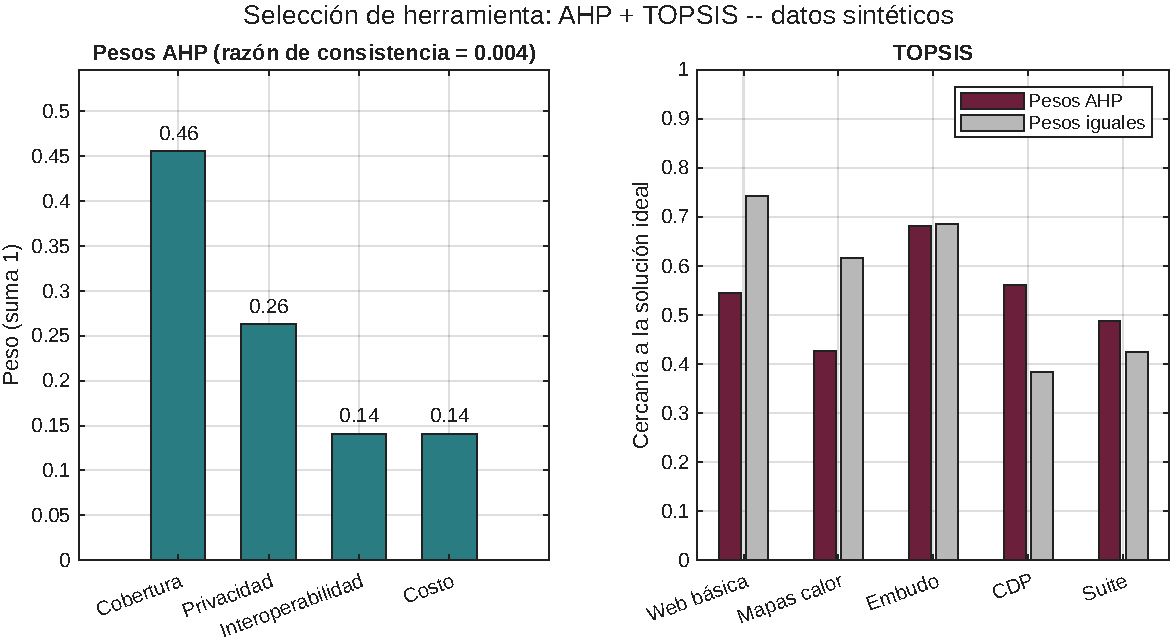
\includegraphics[width=0.95\textwidth]{figuras/matlab/cap09_ahp_topsis.pdf}
  \captionof{figure}{Pesos AHP y cercanía TOPSIS con pesos AHP y con pesos
  iguales. Fuente: elaboración propia con datos sintéticos.}
  \label{fig:cap09-ahp}
\end{center}

\begin{center}
  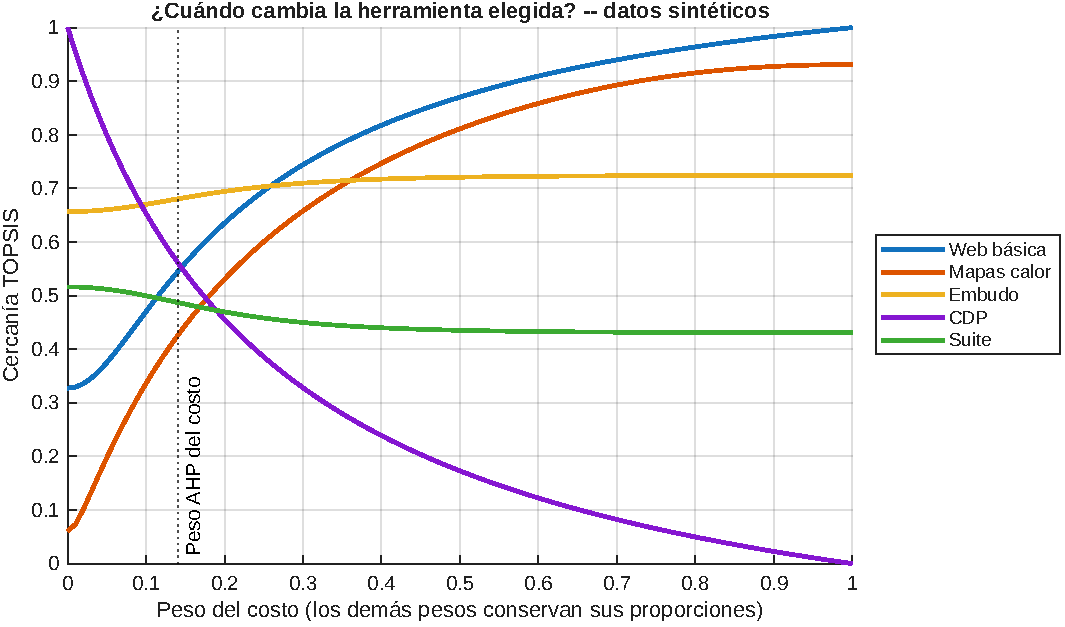
\includegraphics[width=0.88\textwidth]{figuras/matlab/cap09_sensibilidad_costo.pdf}
  \captionof{figure}{Cercanía TOPSIS al variar el peso del costo. Fuente:
  elaboración propia con datos sintéticos.}
  \label{fig:cap09-sensibilidad}
\end{center}

\textbf{Interpretación de negocio.} Con los juicios por defecto, los pesos son
0.455 (cobertura), 0.263 (privacidad), 0.141 (interoperabilidad) y 0.141
(costo), con una razón de consistencia de 0.004: los juicios son coherentes.
TOPSIS elige el tipo \textit{analítica de embudo}. Con pesos iguales, en
cambio, elegiría \textit{analítica web básica}. Los juicios sobre qué importa
más \emph{cambian la elección}, y por eso conviene que cada integrante del
equipo los haga por separado y se discutan las diferencias.

La figura~\ref{fig:cap09-sensibilidad} agrega la lección de método. Si el
peso del costo sube de 0.14 a 0.26, la elección pasa a la herramienta
más barata. Por debajo de 0.09, domina la plataforma más completa y cara. La
decisión no es un número: es un intervalo de pesos en que cada alternativa
gana, y comunicarlo así es más honesto que reportar un ganador único.

\textbf{Ejercicio propuesto (usen exactamente este script, solo cambien el
bloque de parámetros).} Corran el script tres veces y completen un cuadro con
los cuatro pesos, la razón de consistencia, si los juicios son consistentes y
la herramienta elegida:
\begin{enumerate}
  \item \textbf{Caso A — valores por defecto:} los seis juicios tal como
  están.
  \item \textbf{Caso B — el costo manda:} cambien los juicios a
  \texttt{cobVsPriv = 0.333}, \texttt{cobVsInterop = 0.5},
  \texttt{cobVsCosto = 0.2}, \texttt{privVsInterop = 1},
  \texttt{privVsCosto = 0.5} y \texttt{interopVsCosto = 0.333}.
  \item \textbf{Caso C — juicios contradictorios:} cambien los juicios a
  \texttt{cobVsPriv = 5}, \texttt{cobVsInterop = 0.333},
  \texttt{cobVsCosto = 3}, \texttt{privVsInterop = 0.2},
  \texttt{privVsCosto = 3} y \texttt{interopVsCosto = 7}.
\end{enumerate}
Con el cuadro completo, respondan por escrito: en el Caso B, ¿qué peso
domina y qué herramienta gana? En el Caso C, ¿qué dice la razón de
consistencia y qué deberían hacer antes de confiar en la elección? A partir de
sus tres corridas, expliquen por qué un método de decisión multicriterio no
elimina la subjetividad sino que la \emph{hace visible}.

\textbf{Extensión opcional.} Cambien en el script una calificación de
\texttt{matrizDecision} (por ejemplo, la privacidad de la herramienta de
mapas de calor) y describan cómo se mueve el ranking.

\textbf{Sin MATLAB.}
\texttt{matlab/cap09/cap09\_seleccion\_plataforma\_interactivo.html} tiene los
mismos juicios, los casos A, B y C y la matriz de comparaciones dibujada.

\textbf{Con datos propios (extensión opcional).}
\texttt{cap09\_seleccion\_datos\_propios.html}
aplica AHP y TOPSIS a una matriz de decisión propia (hoja «Alternativas»; hojas «Criterios» y «Juicios» opcionales). Se pueden escribir los juicios por pares en la propia página, y la app señala el par de juicios más contradictorio cuando la razón de consistencia pasa de 0.10. Los datos no salen del navegador.
\end{cajaLaboratorio}

\begin{cajaEtica}
Elegir una herramienta de análisis es elegir qué datos se recogerán de
personas que no participaron en la decisión. Tres reglas prácticas. La
\emph{minimización}: capturar solo lo que la pregunta de negocio exige, y
excluir de la grabación los campos sensibles (pagos, contraseñas, datos de
salud). El \emph{consentimiento específico}: avisar y obtener consentimiento
antes de usar grabación de sesiones, y verificar la LFPDPPP vigente al
implementar y no solo al estudiar \parencite{dof_lfpdppp2025}. Algunas
herramientas ajustan lo que miden según el consentimiento
\parencite{google2026ga4consent}. La
\emph{salida}: elegir herramientas que permitan exportar y borrar los datos de
una persona, y conocer cuánto tiempo conservan los datos individuales; por ejemplo, la
retención configurable de 2 o 14 meses de las propiedades estándar de GA4
\parencite{google2026ga4retencion}. Y un criterio que los cuatro del laboratorio no capturan:
una herramienta barata y eficaz que viola la privacidad no es una herramienta
barata.
\end{cajaEtica}

\section{Estudio de caso}
\label{sec:cap09-caso}

\begin{casoFicticio}
Tres personas de una agencia deben elegir una herramienta para analizar el
recorrido de una marca de ropa en línea. La responsable de finanzas considera
que el costo es \enquote{muchísimo más importante} que el resto. La analista de
datos prioriza la cobertura del recorrido. La abogada de la agencia exige que
la privacidad y el consentimiento pesen más que cualquier otro criterio.

Cada una llena por separado la matriz de comparaciones por pares. Al
promediar sus juicios, la razón de consistencia del grupo es 0.17.

\textbf{Preguntas guía.}
\begin{enumerate}
  \item ¿Qué indica una razón de consistencia de 0.17 y qué debería hacer el
  grupo antes de continuar?
  \item Proponga cómo reconciliar los tres juicios: promedio, discusión o
  consenso con rangos. Justifique.
  \item ¿Qué herramientas del laboratorio ganarían con los juicios de cada
  persona por separado y qué enseña eso sobre el análisis de sensibilidad?
  \item ¿Qué decisión debería tomar la agencia si dos herramientas quedan
  empatadas en cercanía pero una exige consentimiento más complejo?
\end{enumerate}
\end{casoFicticio}

\section{Actividades y evidencias del portafolio}

Estas actividades cierran el entregable único de la práctica
\enquote{Recorrido del consumidor digital}.

\begin{description}
  \item[Reporte de investigación] Aplicar los cuatro criterios durables a dos
  herramientas reales que el equipo use o pueda usar, con una fuente por
  criterio y con la fecha de consulta (cuadro~\ref{tab:cap09-categorias}).
  \item[Infografías colaborativas] Integrar en una sola infografía el proceso
  de decisión (Cap.~6), el recorrido (Cap.~7) y las figuras participantes
  (Cap.~8) del caso real del equipo, con las capas y herramientas del
  Cap.~9.
  \item[Solución de casos] Resolver por escrito el estudio de caso de la
  agencia (sección~\ref{sec:cap09-caso}).
  \item[Reporte de práctica] Consolidar el entregable único de la práctica
  \enquote{Recorrido del consumidor digital} (ver \enquote{Prácticas oficiales
  de la unidad} al cierre de esta Parte) e incluir el cuadro de los casos
  A, B y C de este laboratorio.
\end{description}

\section{Ruta de aprendizaje autónomo}

Dos horas de aprendizaje autónomo. Tareas concretas:
\begin{enumerate}
  \item Ejecutar \texttt{cap09\_seleccion\_plataforma\_interactivo.html},
  completar el cuadro de los casos A, B y C y anotar en qué punto cambia la
  elección al mover el peso del costo.
  \item Pedir a otras dos personas del equipo que llenen sus propios juicios
  sin ver los de los demás, y comparar los tres conjuntos de pesos.
  \item Verificar, con fecha de consulta, si la ruta descrita en el recuadro de
  Frontera (plataforma de datos o agentes de IA) sigue vigente o cambió
  desde octubre de 2026.
  \item (Opcional) Con \texttt{cap09\_seleccion\_datos\_propios.html} (opcional), cargar el \textbf{Ejemplo 2} (agencias), reducir la razón de consistencia por debajo de 0.10 y anotar qué juicio hubo que cambiar.
\end{enumerate}

\section{Síntesis}

La base tecnológica para analizar el recorrido se ordena en cuatro capas
(captura, identidad, análisis y activación) y cuatro categorías de herramienta
(mapas de calor y sesiones, analítica de embudo y atribución, plataformas de
datos de clientes, suites de redes y comercio). Ninguna cifra de cuota de
mercado entra en el libro; los criterios sí: cobertura del recorrido,
privacidad y consentimiento, interoperabilidad y costo. Para pasar de criterios
a decisión sirven AHP, que convierte comparaciones por pares en pesos y
verifica su consistencia, y TOPSIS, que ordena por cercanía a la solución ideal.
El resultado correcto no es un ganador sino un intervalo de pesos en que cada
alternativa gana, y toda elección de herramienta es también una decisión
sobre los datos de terceros.

\subsection*{Glosario del capítulo}
\begin{description}
  \item[AHP] Proceso Analítico Jerárquico: obtiene pesos de criterios a partir de comparaciones por pares.
  \item[CDP (plataforma de datos de clientes)] Aplicación que unifica datos de clientes de múltiples fuentes en perfiles persistentes y gobernados.
  \item[Cercanía TOPSIS] Cociente entre la distancia a la peor solución y la suma de distancias a la mejor y a la peor; más alto es mejor.
  \item[Juicio por pares] Parámetros editables del script (\texttt{cobVsPriv}, \texttt{cobVsInterop}, \texttt{cobVsCosto}, \texttt{privVsInterop}, \texttt{privVsCosto}, \texttt{interopVsCosto}): cuántas veces es más importante el primer criterio que el segundo. Rango: real entre 1/9 y 9; los valores menores que 1 invierten la comparación. Los casos didácticos usan valores entre 0.2 y 7.
  \item[Razón de consistencia] Cociente $\mathrm{CI}/\mathrm{RI}$ que mide si los juicios se contradicen; menor que 0.10 se acepta.
  \item[Criterio de costo] Criterio en el que menos es mejor; TOPSIS lo invierte al definir la solución ideal.
  \item[Solución ideal] Combinación hipotética de lo mejor en cada criterio ponderado.
  \item[\textit{Session replay}] Grabación de la sesión de una persona en un sitio.
\end{description}

\subsection*{Autoevaluación}

\textbf{Opción múltiple}

\begin{enumerate}
  \item En AHP, una razón de consistencia de 0.17 indica que:
  \begin{enumerate}
    \item[a)] Los juicios son perfectamente coherentes.
    \item[b)] Los juicios se contradicen y conviene revisarlos. \textit{(correcta)}
    \item[c)] Las alternativas son demasiado parecidas.
    \item[d)] El costo pesa demasiado.
  \end{enumerate}
  \textit{Justificación:} concepto detrás del código, sección~\ref{sec:cap09-lab}.

  \item En TOPSIS, para un criterio de costo, la solución ideal es:
  \begin{enumerate}
    \item[a)] El valor máximo ponderado.
    \item[b)] El valor mínimo ponderado. \textit{(correcta)}
    \item[c)] El promedio.
    \item[d)] El valor de la primera alternativa.
  \end{enumerate}
  \textit{Justificación:} concepto detrás del código.

  \item ¿Cuál de las siguientes es una pregunta de la capa de
  \enquote{identidad y consentimiento}?
  \begin{enumerate}
    \item[a)] ¿Dónde da clic la mayoría?
    \item[b)] ¿La identidad se unifica de forma real o probabilística, y con qué base legal? \textit{(correcta)}
    \item[c)] ¿Cuánto cuesta la licencia?
    \item[d)] ¿Qué color usa el panel?
  \end{enumerate}
  \textit{Justificación:} sección~\ref{sec:cap09-capas}.
\end{enumerate}

\textbf{Preguntas abiertas}

\begin{enumerate}
  \item Explique por qué el capítulo no reporta la cuota de mercado de ninguna
  herramienta. \textit{Clave:} las cifras provienen de blogs de proveedores y
  analistas, no de fuentes primarias verificables, y envejecen rápido; la
  estructura de criterios perdura.
  \item A partir de la figura~\ref{fig:cap09-sensibilidad}, explique por qué
  comunicar un intervalo de pesos es más honesto que reportar un solo
  ganador. \textit{Clave:} los pesos son juicios subjetivos y la elección
  cambia dentro de intervalos; el análisis de sensibilidad lo hace visible.
\end{enumerate}

\section{Lecturas recomendadas}

\begin{description}
  \item[\textcite{saaty1977}] La fuente primaria del AHP. Denso, pero la sección sobre la escala de comparación y el vector propio se lee sin más álgebra que la del capítulo.
  \item[\textcite{hwang1981}] Fuente primaria de TOPSIS y panorama de métodos de decisión multiatributo.
  \item[\textcite{gartner2026cdp}] Evaluación de la categoría CDP. Léase como panorama de analistas y con la cautela del cuadro del Cap.~7 sobre fuentes de consultoría.
  \item[\textcite{anderl2016}] Conecta la analítica de recorridos con la atribución por cadenas de Markov; útil para evaluar si una herramienta ofrece algo más que el último clic.
\end{description}
